% German Rule sheet for primes game
% Game design: Grant Sinclair
% Graphic design: Harald Bögeholz

\documentclass{article}

% For German language
\usepackage[german]{babel} 
\usepackage[T1]{fontenc} 
\usepackage[utf8]{inputenc} 

\usepackage[a4paper, left=5cm, right=5cm, top=3cm, bottom=3cm]{geometry}

\usepackage{fontspec}
\usepackage{graphicx}
\usepackage{adjustbox}

% For custom header and footer
\usepackage{fancyhdr}
\usepackage{datetime}

\pagestyle{fancy}
\fancyhf{} % clear all header and footer fields
\renewcommand{\headrulewidth}{0pt} % no line in header area
\fancyfoot[L]{Schwupps oder Schubs} % left footer
\fancyfoot[C]{\thepage} % center footer
\fancyfoot[R]{\today} % right footer

\setmainfont{HelveticaNeue}

\newcommand{\card}[1]{\adjustbox{valign=m}{\includegraphics[page=#1, width=2cm]{primecards-screen.pdf}}}
\newcommand{\largecard}[1]{\adjustbox{valign=m}{\includegraphics[page=#1, width=45mm]{primecards-screen.pdf}}}
\newcommand{\square}[1]{\adjustbox{valign=m}{
\includegraphics[page=#1, width=2cm]{boardsquares.pdf}}}

\setlength{\parindent}{0pt}

\begin{document}

{\center\LARGE\textbf{Schwupps oder Schubs -- ein Spiel für 2 bis 5 Spieler}}

\section*{Vorbereitung}

Jeder Spieler beginnt mit einem Spielstein auf dem Startfeld. Die Karten werden gemischt. Bei zwei oder drei Spielern erhält jeder zwei Karten, bei vier oder fünf Spielern je drei. Der Kartenstapel wird mit der schwarzen Seite nach oben gelegt. Bei fünf Spielern werden die obersten drei Karten entfernt. Die Spieler sollten ihre Karten so halten, dass nur sie die Symbole auf den weißen Seiten sehen können, aber alle anderen die Zahlen auf den schwarzen Seiten sehen können.

\section*{Spielablauf}

Die Spieler ziehen im Uhrzeigersinn. Wenn Du an der Reihe bist, kannst Du \textbf{schwuppsen} oder \textbf{schubsen}.

\begin{description}

\item[Schwuppsen:] 

Du spielst eine einzelne Karte mit der schwarzen Seite nach oben und ziehst um so viele Felder vorwärts, wie auf der Karte angegeben ist.

\item[Schubsen:]

Du spielst eine beliebige Anzahl von Karten mit der weißen Seite nach oben, sodass die Symbole auf den Karten \textbf{genau} den Symbolen auf einem von einem Gegner besetzten Feld entsprechen. Du schubst den Spielstein des Gegners um die Summe der Zahlen auf den Karten zurück und \textbf{danach} ziehst Du Deinen eigenen Spielstein um die gleiche Anzahl nach vorne. Wenn Du kannst, darfst Du jetzt so oft wie Du möchtest weiter schubsen, darfst aber in diesem Zug nicht mehr schwuppsen. \textbf{Gnadenregel:} Der letzte Spieler darf nicht geschubst werden.

\end{description}

Auf jedem Feld kann nur ein Spielstein stehen. Wenn ein Spielstein auf ein besetztes Feld bewegt wird, wird der andere Spielstein um ein Feld zurückgestupst. Wenn dieses Feld besetzt ist, wird dessen Spielstein um eins zurückgestupst und so weiter. Das einzige Feld, das mehrere Spielsteine aufnehmen kann, ist das Startfeld. Ein Spielstein kann nicht unter Null geschubst werden und bleibt auf dem Startfeld stehen. Die 100 muss exakt getroffen werden; wenn ein Spielstein zu nahe an 100 ist und die gespielte Zahl zu groß ist, muss der Spielstein an Ort und Stelle bleiben.

Am Ende Deines Zugs \textbf{ziehst Du zwei Karten} und legst alle gespielten Karten auf den Ablagestapel. Abgelegte Karten werden nicht wiederverwendet; wenn die Karten aufgebraucht sind, beginnt das Endspiel.

\section*{Spielende}

Wenn ein Spieler 100 erreicht, gewinnt er das Spiel. Wenn die Karten vorher aufgebraucht sind, beginnt das \textbf{Endspiel}: Wenn ein Spieler am Ende seines Zuges Letzter ist, scheidet er aus und nimmt seinen Spielstein vom Brett. Gewinner ist, wer am Ende übrig bleibt.

\section*{Beispiel}

Angenommen, Gelb ist am Zug und der Spielstein von Blau befindet sich auf Feld \square{12} und der von Rot auf Feld~\square{5}.

Gelb schubst, indem er \card{91} \card{69} spielt, insgesamt 7, bringt Blau von Feld \square{12} zurück auf Feld \square{5} und drängt Rot von Feld \square{5} zurück auf Feld \square{4}. Gelb zieht 7 Felder vorwärts.

Gelb schubst nun erneut, indem er \card{125} spielt, und schickt Blau von Feld \square{5} zurück zum Startfeld. Gelb zieht 6 Felder nach vorne und beendet den Zug, legt alle gespielten Karten ab und zieht zwei Karten.

Jetzt ist Rot an der Reihe. Rot spielt~\card{170} und zieht 8 Felder nach vorne, landet also auf Feld~\square{12}. Rot legt die gespielte Karte ab und zieht zwei Karten.

\section*{Kurz-Variante}

Die Regeln sind wie oben, aber das Spiel endet bei 50; die 50 muss exakt getroffen werden. Du kannst das Brett falten und nur die untere Hälfte benutzen.

\section*{Fortgeschrittene Regeln für 2--3 Spieler}

Die Regeln sind die gleichen wie oben mit folgender Abwandlung: Die Gnadenregel gilt nicht. Jeder Spieler hat zwei Spielsteine der gleichen Farbe. Nach dem Mischen wird abgehoben. Der Gewinner ist der Spieler, dessen \textbf{letzter Spielstein bei Spielende am weitesten vorn ist}. Spieler dürfen nur auf die 100 ziehen, wenn sie dadurch gewinnen.

\section*{Teamspiel für 4 Spieler (2 Teams à 2 Spieler)}

Die Regeln sind die gleichen wie die fortgeschrittenen Regeln. Die Spieler sitzen ihrem Partner gegenüber. Partner dürfen keine Strategie miteinander besprechen. Jedes Spielerpaar hat zwei Spielsteine derselben Farbe.

\newpage
\section*{Über die Karten}

Das Deck hat 108 Karten, 12 für jede Zahl von 1 bis 9. Für jede Zahl zeigt die Rückseite (schwarze Seite) der Karte, welche 12 Symbole (oder Kombinationen von Symbolen) auf der weißen Seite der Karten mit dieser Zahl sind.

\begin{adjustbox}{center}
\begin{tabular}{ccc}
\vspace*{5pt}\\
\largecard{2} & \largecard{26} & \largecard{50} \vspace*{10pt}\\
\largecard{74} & \largecard{98} & \largecard{122} \vspace*{10pt}\\
\largecard{146} & \largecard{170} & \largecard{194} \vspace*{10pt}\\
\end{tabular}
\end{adjustbox}

\end{document}
